\chapter{Introduction}
\label{chap:intro}

%%%%%%%%%%%%%%%%%%%%%%%%%%%%%%%%%%%%%%%%%%%%%%%%%%%%%%%%%%%%%%%%%%%%%%%%%%%%%%%
\section{Motivation}
\label{sec:chap1-motivation}


Numerical simulation of neutron physics inside a nuclear reactor is fundamental to the design and operation of nuclear power plants. Neutron physics simulations are necessary for determining core reactivity, power distributions, isotopic depletion, and transient behavior. Accurate and predictive simulations can improve the operation of current nuclear reactors by reducing overly-conservative safety margins, incorporating accident tolerant fuels, and extending to longer operating cycle lengths. In addition, predictive neutron physics simulations are critical to the evaluation of advanced reactor designs, many of which operate in very different physics regimes than currently operating reactors. 

Currently operating nuclear reactors often rely on nodal diffusion methods to simulate neutron physics. These methods are very fast and efficient but have difficulty capturing localized gradients. In current generation nuclear reactor designs, such as the Westinghouse AP 1000\texttrademark \ac{PWR}, there is much greater geometric and material complexity than previous generations. These new complexities such as axial enrichment zoning and partial length \acp{BP} allow for greater efficiency and longer cycle lengths by reducing power peaking. However, the increase in axial heterogeneity poses significant issues for nodal methods. Specifically, nodal diffusion solvers often assume smooth axial variation of scalar flux distributions within fuel assemblies. Therefore, these complex features  lead to axial and radial profiles which are not smooth enough for modern nodal methods to be accurate.

While higher fidelity methods are capable of resolving local gradients and fine heterogeneous detail, they are often significantly slower. This can be prohibitive in reactor analysis where many simulations are required in a relatively short time frame. The goal of high fidelity modeling in this realm is to create a tool that can benchmark and inform the development of nodal diffusion solvers. Even as a benchmark tool, high fidelity neutron physics simulations can be too computationally intense to be useful. Therefore, there is a need for 3D high fidelity neutron physics simulations that are accurate and reliable but also computationally efficient. This thesis focuses on developing a high fidelity 3D \ac{MOC} solver capable of forming benchmark solutions in reasonable computational time.

%%%%%%%%%%%%%%%%%%%%%%%%%%%%%%%%%%%%%%%%%%%%%%%%%%%%%%%%%%%%%%%%%%%%%%%%%%%%%%%
\section{Background}
\label{sec:chap1-background}

Nodal methods are the standard for full core neutron physics simulation in modern reactor analysis. In order to form reasonable solutions, these simulations rely on accurate multi-group cross-section data formed from a multi-level approach to decouple the energy, angular, and spatial dimensions as depicted in Figure~\ref{fig:multi-level}~\cite{boyd2017thesis}. The multi-level approach typically combines high-fidelity models of energy self-shielding physics with low fidelity geometric models of unique core components. The energy complexity is then reduced as larger geometric models are considered.

\begin{figure}[ht!]
	\centering
	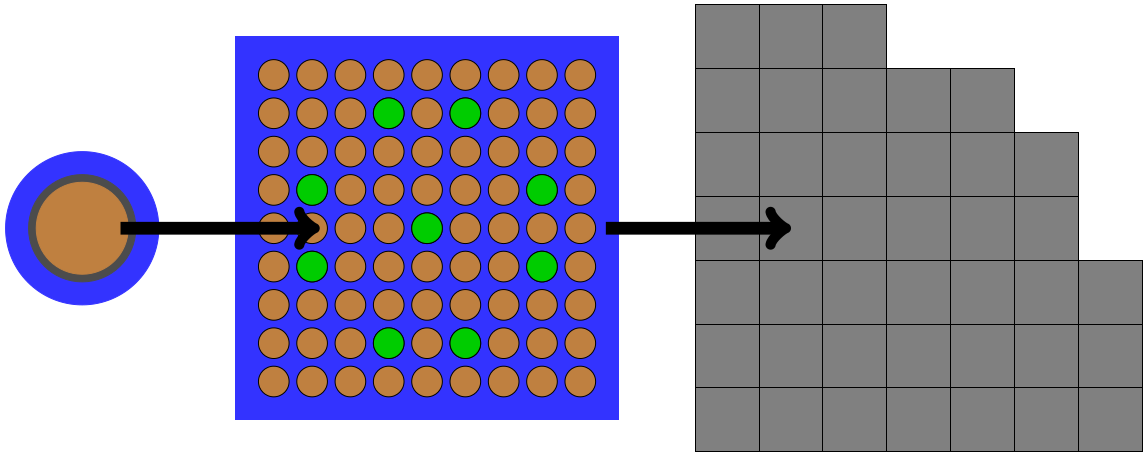
\includegraphics[width=\linewidth]{figures/intro/multi-step-flow-chart.png}
	\caption{A depiction of the current multi-level simulation process for full core reactor analysis}
	\label{fig:multi-level}
\end{figure}

The first stage of typical \ac{LWR} multi-group cross-section generation attempts to capture self-shielding effects within an infinite array of fuel pins. This step typically condenses the continuous energy behavior of cross-sections to a $\approx 100$ energy group cross-section set. The next stage captures self-shielding effects between pins by using this cross-section set to simulate every unique fuel assembly within an infinite lattice, further reducing the group structure to a few group cross-section set. Lastly, these cross-sections are used in a full core nodal diffusion solver where the neutron behavior over each assembly is homogenized. The resulting coarse mesh solution is then superimposed on the individual single assembly solution to reconstruct pin-powers.

Every step of the multi-level approach introduces assumptions and approximations. In order to develop a high fidelity neutron transport simulation tool, these approximations should be removed. Monte Carlo simulations incorporate minimal approximations and are often viewed as the gold standard for accurate neutron physics simulation. However, an extremely large number of Monte Carlo histories is required to produce accurate pellet-level fission rates, leading to a very large computational cost.

An alternative approach can be taken whereby the full core is directly simulated by many-group transport methods. The multi-group cross-sections can be formed from direct Monte Carlo simulation of the full core problem where reaction rate tallies within regions are used to form accurate approximations of the multi-group cross-sections. Since these cross-section tallies can converge significantly faster than pin powers using machine learning techniques~\cite{boyd2017thesis}, the computational cost can be significantly reduced. 
%While approximations are still introduced during the formation of these multi-group cross-sections, the significant approximations introduced from nodal method diffusion methods are removed.

While the use of transport methods in place of nodal diffusion methods leads to a dramatic increase in computational requirements for reasonable solutions, recent advances in computational power for both engineering clusters and large scale supercomputers have enabled the computation of extremely large scale reactor simulations. 

One such transport method is \ac{MOC}, which discretizes the neutron transport equation using many characteristic paths and directions which traverse the reactor geometry. \ac{MOC} has seen widespread use for the 2D lattice physics analysis of single assemblies, as described previously in the multi-level approach. Additionally, 2D radial core slices of reactor geometries have been simulated using \ac{MOC}. However, for reactors with significant axial heterogeneity, 3D methods should be used to capture the axial detail. 

Due to the computational expense of direct full core 3D deterministic neutron transport methods, many have focused on 2D/1D methods~\cite{2d1d,liu2d1d, tang2d1d, collins2d1d, jarrett2d1d, wenbin2d1d} which solve 3D problems as a coupled system of radial and axial transport problems. A chosen number of radial slices are simulated with some 2D transport method, such as 2D \ac{MOC}. Transverse leakage terms couple the radial problems through a 1D transport or diffusion method. While this approach reduces the computational burden in comparison with direct 3D transport simulations, it also introduces approximations. Instead, the work in this thesis focuses on explicitly solving the 3D deterministic neutron transport equations with \ac{MOC}.

%%%%%%%%%%%%%%%%%%%%%%%%%%%%%%%%%%%%%%%%%%%%%%%%%%%%%%%%%%%%%%%%%%%%%%%%%%%%%%%
\section{Literature Review of 3D MOC}
\label{sec:lit-review}

Previously, others have attempted to simulate reactor physics problems using 3D \ac{MOC} but have been limited to small models due to computational constraints of their particular 3D \ac{MOC} implementations. Therefore, this thesis concentrates on efficiently solving the 3D \ac{MOC} system of equations in order to make full core calculations feasible. Here, a variety of past and present 3D \ac{MOC} implementations are discussed and compared with the OpenMOC implementation presented in this thesis.

\subsection{DRAGON}
\label{sec:dragon}
DRAGON is a neutron transport code concentrating on lattice physics calculations for CANDU reactors. Since CANDU reactors contain fuel elements with reactivity control devices placed perpendicularly to the fuel channels, accurate calculations require full 3D treatment of the physics. Therefore, a 3D \ac{MOC} solver was implemented, named MCI~\cite{dragon_3d_moc}. 

MCI solves the flat source \ac{MOC} equations using a nested iterative process. In outer iterations, the fission source is updated along with the eigenvalue estimate. During inner iterations, the scattering source is updated and transport sweeps yield currents and fluxes. Outward currents are tallied at boundaries with an albedo boundary condition yielding new inward angular fluxes for the following inner iteration. Acceleration is provided with a self-collision rebalancing scheme in which the energy distribution is recalculated during every inner iteration.

A track merging technique was also implemented in which tracks crossing the same regions in the same order are merged. While this may be useful for simple geometries, there would not be many tracks which have the same crossings in complex geometries. Typical full core problems have many radial complexities, reducing the effectiveness of this scheme.

Distributed memory parallelism was also introduced into MCI~\cite{dragon_parallel} in which each process received a copy of all scalar fluxes and a group of tracks to handle. After completing each transport sweep, a global reduction communicates flux information through a sum operation on every region. Angular fluxes were also communicated through global broadcasts. In order to optimize load balancing, many partitioning schemes for the tracks across processes were tested. While the parallel efficiency was decent for the tested cases, the largest case only used 8 CPU cores. For the time of the tests, this was standard. However, for modern parallel computing, this number of cores is quite small, especially for large scale neutron transport calculations.

\subsection{MOCFE}
\label{sec:mocfe}

MOCFE is a finite element \ac{MOC} code created at Argonne National Laboratory~\cite{mocfe_init}. Using a finite element approach, the \ac{MOC} system of equations with a flat source approximation are solved in matrix form. The iteration scheme consists of iterations over between-group and within-group components. In this nested iteration scheme, the inner iterations iteratively converged the within-group flux solution. Each inner iteration is a transport sweep. Though this scheme is not unusual, it does increase the number of transport sweeps needed to converge the problem.

MOCFE also does not link tracks at boundaries. Due to this implementation decision, approximations are required to treat reflective or periodic boundary conditions. However, the lack of track linking requirements allows for less constraints when constructing a quadrature set. MOCFE implements a quadrature set in which projections to spherical harmonics of the scattering kernel are exactly preserved. Tracks are also created symmetric in $z$ with each track representing both forward and backward angular fluxes.

The parallelism in MOCFE is implemented with \ac{MPI}~\cite{mpi} parallelization over trajectories such that each process receives a copy of all source regions. On every transport sweep, each process computes the variation of angular fluxes over its trajectories and accumulates their contribution to all source regions. In order to communicate the results, global reductions are required at the end of each transport sweep, which can be quite expensive.

Application of MOCFE to large scale problems distributed across many processors was studied at length~\cite{mocfe_bgp}. In order to increase scalability, the entire space, angle, and energy variables were decomposed across \ac{MPI} processes. While this does indeed increase the parallelism, it can lead to dramatically inefficient designs due to poor cache efficiency. In this thesis, energy groups for a given computation are always treated in the same task in order to increase performance.

The decision to explicitly store \ac{MOC} information in matrices can also lead to poor performance. Typical efficient \ac{MOC} implementations implicitly compute matrix elements of the transport equations on-the-fly rather than storing the data in some typical matrix representation.  MOCFE uses a \ac{GMRES} linear solver to solve the \ac{MOC} equations. While \ac{GMRES} can be quite efficient for arbitrary matrices, the  \ac{MOC} application is quite unique in which matrices can be easily inverted in a transport sweep due to the matrix structure. A \ac{GMRES} implementation oblivious to this structure can incur significant overhead.

Since the computational demands of MOCFE were too large in comparison with other neutron transport simulation tools, the 3D \ac{MOC} solver was abandoned when the code was merged into the PROTEUS neutron simulation suite. Instead of using a 3D \ac{MOC} solver, the code was re-purposed to solve the transport equations using 2D/1D methods in PROTEUS-MOC~\cite{proteus}.

\subsection{MMOC}
\label{sec:mmoc}

Liu created a 3D \ac{MOC} implementation based on modular ray tracing~\cite{liu_mrt} named MMOC. His track laydown algorithm, which allows natural track linking over modular domains, is used in this thesis and thoroughly discussed in Chapter~\ref{chap:track-laydown}. This track laydown is efficient with only slight adjustments needed from desired user parameters, allowing for greatly reduced computational costs in comparison with other track laydown methods which are less flexible and require extra tracks to be inserted in order to ensure track linking at boundaries~\cite{shaner-laydown}. By considering entire 2D cycle lengths rather than individual 2D track lengths when forming track linking relationships, the requirements are significantly less stringent, allowing for the added flexibility.

In this thesis, the modular ray tracing algorithm for track generation is useful for linking tracks at domain boundaries during domain decomposition across many nodes. However, Liu used the modular tracking mainly to reduce ray tracing costs. MMOC approaches the \ac{MOC} problem by splitting it into many modules. Over many of the modules, Liu notes that the geometry and track laydown are the same. Therefore, \textit{typical cells} are identified and ray tracing is only computed for unique cells. For applications in this thesis, ray tracing costs can be trivial in comparison with the overall work of solving the \ac{MOC} equations so the ray tracing aspect of MMOC is less applicable.

%The MMOC implementation also allows for arbitrary order adjusted level symmetric quadratures. First, MMOC creates desired angles and ray spacing to accommodate a level-symmetric scheme. These desired values are then adjusted to ensure linking at module boundaries. Weights are also recalculated with the new angles.

% MMOC was tested on a variety of problems and used \ac{CMFD} acceleration to reduce the number of required iterations to achieve convergence.  However, it appears that the algorithm was only tested on Cartesian problems, lacking any curved surfaces. Since reactor physics problems most commonly involve fuel pins which are cylindrical, these test problems were over-simplified. Since the Cartesian geometries can easily be decomposed into blocks, many having identical geometries, the reuse of ray tracing data would provide more benefit than that expected on a realistic problem. Full core problems also typically have complex radial geometries, including such features as intermediate grid spacers, core baffles, and many curved surfaces. Therefore, the method of ray tracing only unique cells is not implemented in OpenMOC. However, the method for generating tracks to link at boundaries is quite useful.

\subsection{MPACT}
\label{sec:mpact}

Kochunas implemented a 3D \ac{MOC} solver in MPACT~\cite{mpact_initial, kochunas}, the standard neutron transport code in the VERA core simulator~\cite{vera}.  This was the first 3D \ac{MOC} solver implemented with the intention of solving full core PWR problems with full geometric detail. The solver used many of the common principles and structure of 2D \ac{MOC} solvers at the time. For instance, it used a flat source approximation and explicitly stored segment information during a pre-processing ray tracing step at the beginning of the solver. Unlike other solvers, it used a strict source iteration scheme without any inner iterations. 

The track laydown implemented in the 3D \ac{MOC} solver relied on the Modular Ray Tracing scheme~\cite{liu_mrt}. However, simplifications were made leading to the s-MRT method, discussed further in Chapter~\ref{chap:track-laydown}. One of the reasons presented for these simplifications was to avoid tracks intersecting corners. In OpenMOC, corner intersections are allowed and are explicitly treated. While the s-MRT method leads to a much simpler track laydown algorithm, it has serious drawbacks. Specifically, the axial ray spacing must be finer than the radial ray spacing. This is problematic for full core \ac{PWR} problems in which there is much greater geometric detail in the radial direction than the axial direction. This can lead to an artificial increase in the number of tracks required to resolve typical \ac{PWR} problems. Since the computational cost (both in memory usage and run time) scales linearly with the number of tracks, any large artificial increase in the number of tracks can significantly hinder the computational performance. Published MPACT results show only a modest artificial increase (~8\%) in the number of tracks, but a fine axial ray spacing was assumed to be necessary. Published results for OpenMOC~\cite{shaner-laydown, openmoc-beavrs} show that it is possible to significantly coarsen the axial ray spacing while maintaining solution accuracy.

One of the benefits of using a modular ray tracing track laydown is the ability to naturally link tracks at domain boundaries when using spatial domain decomposition. The 3D \ac{MOC} solver in MPACT implemented both spatial domain decomposition and angular domain decomposition using non-blocking \ac{MPI} communication~\cite{mpi}. For spatial domain decomposition, the geometry is decomposed into $N$ sub-domains where $N$ is equal to the number of \ac{MPI} processes per number of angular decompositions. An algorithm is implemented to subdivide the geometry in order to maximize the volume-to-surface area ratio of each sub-domain, reducing the relative communication costs which scale with surface area. For angular domain decomposition, each \ac{MPI} process replicates the scalar fluxes of the associated sub-domain, using global reductions to sum all of the tallied contributions to local scalar fluxes across all processes. This reduction operation was shown to be a bottleneck in the parallel scalability of the algorithm.

During each transport sweep, the sweeping algorithm first loops over energy groups, then over angles within the angular sub-domain, then over all tracks within the angular sub-domain in parallel using OpenMP. In this shared memory parallelism implementation, each thread receives a full copy of the scalar fluxes within the sub-domain. This replication of information allows contention between threads to be reduced, but also greatly increases the memory footprint of storing scalar fluxes. In addition, a reduction operation is required to sum together all of the local thread scalar fluxes.

%The choice to loop over energy groups on the outside (rather than on the inner-most loop) causes decreased vectorization. The choice to also loop over angles on the outside and only parallelize over tracks within an angle (rather than parallelizing over all tracks) reduces the potential for parallelism

%During transport sweeps, each track represents both forward and backward directed angular fluxes, a common feature of 2D \ac{MOC} algorithms~\cite{kochunas2007twoway}. When computing the angular flux variation over each source region, the exponential computation is performed using a table interpolation.

\ac{CMFD} acceleration was implemented in MPACT using the \ac{GMRES} linear solver in PETSc with a block ILU preconditioner to solve the associated linear system. The solver was domain decomposed spatially and a procedure was implemented to update angular fluxes at sub-domain boundaries~\cite{mpact_dd_cmfd}.

Various benchmarks were evaluated for the MPACT 3D \ac{MOC} solver. These benchmarks include the Takeda benchmark~\cite{takeda} and the C5G7 benchmark~\cite{c5g7}. Unfortunately, the results did not seem to match well with the reference solution. To understand performance on realistic \ac{PWR} problems, a realistic \ac{PWR} assembly was constructed and modeled. 

A theoretical computational performance model was developed, showing a very high computational cost for full resolving a full core \ac{PWR} problem using the MPACT implementation of 3D \ac{MOC}.

\subsection{APOLLO3}
\label{sec:apollo3}

APOLLO3 is a nuclear reactor analysis code which recently incorporated a 3D \ac{MOC} solver named TDT~\cite{Sciannandrone2016}. TDT solves the \ac{MOC} equations in a nested iterative process, much like the MCI solver in DRAGON. However, TDT adds another layer of iterations. In the outer iterations, new fission sources are computed. Within each outer iteration, thermal iterations are performed in which the scattering source is recomputed. Within each thermal iteration, internal iterations are conducted in which the spatial distribution is resolved. These innermost iterations require computing transport sweeps at every step. This nested iterative process is not implemented in OpenMOC since it increases the number of transport sweeps per fission source calculation. 

One of the main differences between TDT and other \ac{MOC} solvers is the explicit treatment of boundaries. TDT classifies boundaries as open or closed. At open boundaries the angular flux is known. For example, at vacuum boundaries the incoming angular flux is known to be exactly zero. At closed boundaries, such as reflective or periodic boundaries, the angular flux is unknown. Whereas solvers such as OpenMOC treat closed boundaries by estimating the angular flux as being the value from the previous iteration, TDT explicitly computes the angular flux at boundaries by following tracks from an open boundary (where the angular flux is known) along a connecting cycle until it reflects onto the track of interest.

This boundary treatment is of course not possible if the geometry is encompassed entirely by closed boundaries. In these cases, TDT guesses an initial angular flux and follows the track cycle until the initial guess becomes irrelevant. It is unclear whether this is only implemented for cases with all closed boundaries or if this technique is used more generally.

Another critical feature of TDT is the \ac{CCM}. In this method, storage requirements are reduced by characterizing segments (or chords) into different groups: horizontal, vertical, and mixed. For horizontal and vertical chords, their lengths can trivially be computed, and are referred to as \textit{recognized chords}. In addition, all recognized chords of the same type (horizontal or vertical) of the same region will have the same length. Some mixed chords may become recognized chords under certain circumstances, but it is far more difficult than horizontal or vertical chords.

During an initial ray trace, the tracking information is compactly stored in Hit Surface Sequences, which only detail the type of intersections a track observes. These sequences, which only consist of one integer per segment or chord, can determine both the type of intersections encountered (recognized or unrecognized) as well as the regions which the segments overlap.

For all unrecognized chords, segment lengths as well as exponential terms are computed and explicitly stored. During transport sweeps, they are simply loaded from memory. For all recognized chords, their segment lengths and exponential terms are computed on-the-fly during the transport sweeps with no upfront storage of segment information. Before the transport sweep an interpolation table is stored for the exponential term. During the transport sweep, this table is used for the computation of exponential terms for recognized chords. 

Some ideas of \ac{CCM} are implemented in OpenMOC. For instance, OpenMOC identifies vertical and horizontal chords in order to efficiently ray trace. However, other features of \ac{CCM} are not implemented. For instance, the effectiveness of the storage technique relies on many recognized chords. Many of the tests conducted on \ac{CCM} have a high ratio of axial source height to axial ray spacing, therefore having many recognized chords, and yielding favorable computational results. However, our previous tests have shown that for coarse axial source height, the axial ray spacing can also be coarsened, lowering the number of potential recognized chords.

%Adds "special directions" (completely vertical, completely horriztonal) to quadrature

%groups on outside

Initially, the TDT solver was dependent on a flat source approximation. Its accuracy was verified on a variety of benchmark problems~\cite{apollo3_3dmoc, apollo3_vv}. More recently, it has been extended to allow for axial polynomial expansions of the source~\cite{apollo3_extruded}. The radial variation of the neutron source within each source region is still assumed to be flat. The authors cite radial heterogeneity and complexity for not using a higher order source approximation in the radial plane. The higher order source approximation requires significantly more computational work per segment but allows a much coarser axial mesh to be used. \ac{CCM} is emphasized for its ability to mitigate the additional work required for the higher order source approximation as it allows for chords of equal lengths to be efficiently computed. While developed for arbitrary order axial polynomial expansions, the published results focus on quadratic axial sources.

The TDT implementation is parallelized with OpenMP. The work is divided in a task-based parallelism approach. Each thread receives a set of tracks and a full copy of the scalar flux accumulators. When a given thread changes angle, the local copy of scalar flux accumulators are synchronized with the global scalar flux accumulator. Since this synchronization can be a bottleneck for parallel scaling, tracks are sorted into groups to minimize the frequency of changing angle.

The TDT implementation has also recently extended its capabilities by adding $DP_n$ synthetic acceleration which supports polynomial flux fields~\cite{apollo3_exp}. This is perhaps the first publication of explicitly treating higher order source components with acceleration techniques. In OpenMOC, the higher order source components are not directly treated during acceleration. Instead, both flat and high order source components are updated together during the prolongation stage of the acceleration.

\subsection{CACTUS}
\label{sec:cactus}

CACTUS was one of the first developed 2D \ac{MOC} neutron transport simulators~\cite{cactus_2d}. It is part of the WIMS core physics simulator and has been the standard lattice physics code used by the simulator for over 20 years. Recently, a 3D \ac{MOC} solver named CACTUS3D was added~\cite{cactus_3d}, reusing much of the CACTUS code. 3D geometry and ray tracing abilities were added for CACTUS3D, with much of the framework of the flux solver imported from CACTUS. Since CACTUS3D observed significant changes in track laydown for small changes in tracking parameters, a new 3D \ac{MOC} solver was created as the main simulation tool in WIMS for solving core calculation~\cite{cactus_wims}. This solver is named  CACTUSOT since rays are treated in a ``once-through'' approach.

In the once-through scheme, each track assumes zero incoming angular flux and is only followed until it reaches the boundary of the geometry. Therefore this approach is limited to core problems with vacuum boundaries. Since tracks do not pass their angular fluxes to other tracks, as would be the case in problems with reflected boundaries, a cyclic track laydown with track linking at boundaries does not need to be enforced. Instead, tracks are generated to uniformly fill the geometry. This is accomplished by generating parallel tracks at every angle on each boundary surface, separated by constant spacing in all directions. This approach was largely adopted due to concerns over untracked elements and calculation of element volumes.

Both CACTUS3D and CACTUSOT explicitly save tracking data for segments. Whereas CACTUS3D stores tracking information for \textit{every} segment, CACTUSOT uses a slice-based geometry treatment. In this approach, the geometry is split into different slices. Each slice represents the geometry over a certain axial interval. In common reactor problems there might only be a few unique slices. Tracks are generated on each slice rather than the full problem and the tracking data is only stored for each unique slice. 

Since tracks are generated for each slice and are not guaranteed to align at slice interfaces, this creates an issue for determining connecting angular fluxes. This is overcome by using track cross-sectional area and outward-directed angular fluxes to compute leakage rates out of the slices on each radial mesh cell on the interface boundary. Inward-directed angular fluxes are then computed by using tack cross-sectional areas and the computed leakage rates.

CACTUSOT also implements features found in CACTUS including \ac{CMFD} acceleration restricted to Cartesian mesh, treatments for both transport-corrected P0 and anisotropic P1 scatter, and a diamond difference representation of the neutron source along track segments. Parallelism is introduced with \ac{MPI} in which work is decomposed by track direction.


\section{The LEAF Method}
\label{sec:leaf}

A successor to the ASMOC3D method~\cite{pre_leaf}, the LEAF method~\cite{leaf_init, leaf_method} approaches the 3D \ac{MOC} problem in a very unique manner. Instead of basing the method on characteristic lines, vertically oriented characteristic planes are used instead. These methods ray trace over certain axial zones, much like a 2D/1D method, assuming an axially extruded geometry in which every radial plane has the same meshing. The vertically oriented characteristic planes are chosen to link at interfaces -- both between axial zones and between connecting planes along the same radial direction within the current axial zone. In the LEAF method, the angular flux at interfaces is represented with a 2nd order Legendre expansion.

The equations are cast in terms of collision probabilities, escape probabilities, and transmission probabilities for the planes. Numerical integration is applied for each characteristic plane in order to determine these probabilities. This numerical integration is accomplished by laying axially stacked tracks across the plane for a given polar angle. These tracks form the abscissa of the integration. 

At this point, the method described is very similar to 3D \ac{MOC}. Aside from the angular flux being represented at interfaces by a 2nd order Legendre expansion, the numerical integration by laying axially stacked tracks in the plane causes the method to be equivalent to filling the geometry full of characteristic lines. It is essentially a re-working of the equations to cast the problem in a different context.

However, the main difference for practical application comes when these probabilities are computed as part of a pre-processing step. Rather than explicitly computing the probabilities (collision, escape, and transmission) of all vertical planes in the problem, the probabilities are computed and tabulated for a range of conditions and interpolated during transport sweeps. The interpolation parameters are: polar angle, axial height of the vertical plane, radial thickness, and total cross-section. By creating the lookup tables only using the chosen abscissa, the amount of work can be greatly reduced.

Since the goal of this method is to treat coarse axial regions, higher order source approximations are introduced. Specifically, sources are formed up to 2nd order in the axial direction and first order in the radial direction. These higher order source approximations allow for a significantly coarsened mesh while maintaining accuracy, reducing the computational requirements of the method.

So far the method has only been tested on somewhat small problems. However, it shows great potential. As long as the required probabilities can be accurately interpolated from somewhat coarse abscissa and the 2nd order Legendre approximation of angular flux is sufficiently accurate, this method should outperform 3D \ac{MOC} methods. However, if a very large number of abscissa are required or the 2nd order Legendre approximation is not sufficient, then explicit 3D \ac{MOC} methods would be preferable. 


%%%%%%%%%%%%%%%%%%%%%%%%%%%%%%%%%%%%%%%%%%%%%%%%%%%%%%%%%%%%%%%%%%%%%%%%%%%%%%%
\section{Objective}

This thesis seeks to develop an efficient 3D \ac{MOC} solver which can solve large 3D reactor physics problems. The behavior of 3D \ac{MOC} and the sensitivity of its solution to input parameters, such as mesh refinement, is studied on a variety of realistic reactor physics problems. However, the primary goal of this thesis is to directly use 3D \ac{MOC} to accurately and efficiently simulate full core \ac{LWR} problems. While simulation accuracy is highly dependent on input cross-section data, accuracy in this context refers to fully converging the problem in both space and angle for a cross-section set which allows for reasonable accuracy. The computational scale of full core \ac{LWR} problems is extremely large with approximately 100 billion region-wise unknowns, assuming a 70 group cross-section library with a geometry defined by a $17 \times 17$ assembly lattice, each with $17 \times 17 \times 200$ pin-cells, and each pin-cell containing 24 source regions with one average scalar flux and three scalar flux moments for each group in each source region. Additionally, the angular space must be sufficiently covered for each region, leading to approximately 100 trillion angular-dependent unknowns for a segment density of ten thousand segments per source region.

%%%%%%%%%%%%%%%%%%%%%%%%%%%%%%%%%%%%%%%%%%%%%%%%%%%%%%%%%%%%%%%%%%%%%%%%%%%%%%%
\section{Thesis Outline}

This thesis starts with an introduction to the \ac{MOC} method and derives its associated equations in Chapter~\ref{chap:moc}. The traditional flat source approximation is discussed and a 3D track-based linear source approximation is introduced. Then, the implementation of the \ac{MOC} algorithm in OpenMOC is discussed.  An emphasis is placed on how the implementation aspects allow for computational efficiency. Chapter~\ref{chap:software-design} introduces the software design of OpenMOC and how the internal structure was re-designed to accommodate 3D \ac{MOC} methods studied in this thesis. Chapter~\ref{chap:track-laydown} discusses the efficient modular track laydown which reduces the total number of tracks required to converge common reactor physics problems. Chapter~\ref{chap:ray-tracing} discusses the on-the-fly ray tracing used in OpenMOC to reduce the total memory footprint and increase cache efficiency. Chapter~\ref{chap:domain-decomposition} discusses the efficient spatial domain decomposition introduced for both the \ac{MOC} and \ac{CMFD} solvers in OpenMOC.

With these components allowing for efficient computation, the convergence aspects of \ac{MOC} are studied, illuminating issues with the traditional source iteration process with transport-corrected cross-sections. Significant discussion is given to the iteration process used to converge the equations from a linear algebra perspective. A diagonal stabilization fix is introduced in Chapter~\ref{chap:moc-convergence} which alleviates the convergence issues through damping of \ac{MOC} flux updates. The effect of \ac{CMFD} acceleration is also discussed. 

Finally, simulation results of OpenMOC are presented on \ac{PWR} geometries. Chapter~\ref{chap:moc-sensitivity} conducts sensitivity studies of \ac{MOC} parameters on cut-outs of the BEAVRS benchmark. The optimal parameters are then used in Chapter~\ref{chap:full-core-results} for full core simulations of the BEAVRS benchmark. Resulting fission distributions are compared with an OpenMC reference solution and slight sensitivity studies are also conducted for the full core in order to ensure the chosen \ac{MOC} parameters sufficiently converge the full core fission distribution. The thesis ends with a summary of progress made in this research for full core deterministic transport methods in Chapter~\ref{chap:conclusions}.